\documentclass{article}
\usepackage[T1]{fontenc}
\usepackage[utf8]{inputenc}
\usepackage{ismir,amsmath,cite,url}
\usepackage{graphicx}
\usepackage{color}
\usepackage{booktabs}
\usepackage{framed}

% Typographical niceties
\usepackage[british]{babel}
\usepackage{csquotes}
\usepackage{microtype}
\usepackage{balance}
\usepackage{enumitem}
\usepackage{newtxmath}
\usepackage[bookmarks=false,hidelinks]{hyperref}

\newcommand{\subfiglabel}[1]{(\textbf{\textsc{#1}})}

\title{Mode Classification and Natural Units in Plainchant}

\oneauthor
{Bas Cornelissen \hfil Willem Zuidema \hfil John Ashley Burgoyne}
{Institute for Logic, Language and Computation, University of Amsterdam 
    \\{\url{mail@bascornelissen.nl}, \url{zuidema@uva.nl}, \url{j.a.burgoyne@uva.nl}}
}

\sloppy
\begin{document}
%
\maketitle
%
\begin{abstract}
Many musics across the world are structured around multiple \emph{modes}, which hold a middle ground between scales and melodies. 
We study whether we can classify mode in a corpus of 20,865 medieval plainchant melodies from the Cantus database.
We revisit the traditional `textbook' classification approach (using the final, the range and initial note) as well as the only prior computational study we are aware of, which uses pitch profiles.
Both approaches work well, but largely reduce modes to scales and ignore their melodic character.
Our main contribution is a model that reaches 93--95\% $F_1$ score on mode classification, compared to 86--90\% using traditional pitch-based musicological methods. Importantly, it reaches 81--83\% even when we discard all absolute pitch information and reduce a melody to its contour.
The model uses tf--idf vectors and strongly depends on the choice of units: i.e., how the melody is segmented.
If we borrow the syllable or word structure from the lyrics, the model outperforms all of our baselines. 
This suggests that, like language, music is made up of `natural' units, in our case between the level of notes and complete phrases,  a finding that may well be useful in other musics.
\end{abstract}



%=============================================
\section{Introduction}\label{sec:introduction}
%=============================================



In his seminal Grove entry, Harold Powers \cite{Powers2001} points out a remarkable cross-cultural generalisation: many musics are structured around multiple \emph{modes}.
Modes are often associated with the major--minor distinction in Western music, but there are much richer systems of modes:
examples include Indian \emph{raga}, Arabic \emph{makam}, Persian \emph{dastgah}, \emph{pathet} in Javanese gamelan music and the \emph{modes} of Gregorian chant.
The specifics obviously vary, but all these phenomena share properties with both scales and melodies, and are perhaps best thought of as occupying the continuum in between \cite{Powers2001}.
On the one hand, a mode is more than a scale: it might imply a hierarchy of pitch relations or favour the use of characteristic motifs.
On the other hand, it is not as specific as a particular tune: a mode rather describes a melody \emph{type}.
Modes are of central importance to their musical tradition, both as means to classify the repertoire, and as practical guides for composition and improvisation \cite{Powers2001}.
Characterising modes computationally is therefore an important problem for \emph{computational ethnomusicology}.


Several \textsc{mir} studies have investigated automatic mode classification in Indian \emph{raga} \cite{Chordia2007,Gulati2016a}, Turkish \emph{makam} \cite{Unal2012,Atalay2020} and Persian \emph{dastgah} \cite{Abdoli2011,Heydarian2019}.
These studies can roughly be divided in two groups.
First, studies emphasising the scalar aspect of mode usually look at pitch distributions \cite{Chordia2007,Atalay2020,Heydarian2019}, similar to key detection in Western music.
Second, studies emphasising the melodic aspect often use sequential models or melodic motifs \cite{Unal2012,Gulati2016a}.
For example, \cite{Unal2012} trains $n$-gram models for 13 Turkish makams, and then classifies melodies by their perplexity under these models.
Going beyond {$n$-grams}, \cite{Gulati2016a} uses motifs, characteristic phrases, extracted from raga recordings to represent every recording as a vector of motif-frequencies.
They weigh counts amongst others by the \emph{inverse document frequency} (see section \ref{sec:tfidf}), which balances highly frequent motifs, and favours specific ones.


In this paper, we focus on automatic mode classification in Medieval plainchant.
This has only rarely been studied computationally, even though the term (if not the phenomenon) `mode' originates there.
At first glance, mode in plainchant is relatively clear, though certainly not entirely unambiguous.
With a second glance, it has a musicological and historical depth that inspired a vast body of scholarship going back over one thousand years.
The music is indeed sufficiently distant in time from most other musics, including Western classical and pop music, to provide an interesting cross-cultural comparison.
And for once, data is abundant, thanks to the immense efforts of chant scholars.


Chant has mostly figured in \textsc{mir} studies in optical music recognition of medieval manuscripts:
the \textsc{simssa} project, for example, has used such systems
to transcribe plainchant from the Cantus database \cite{Helsen2014}.
Recent \textsc{ismir} conferences have also included analyses of Byzantine plainchant \cite{Panteli2013} and Jewish Torah tropes \cite{vanKranenburg2011}, and a comparison of five Christian chant traditions using interval $n$-grams \cite{vanKranenburg2017}.
But, to the best of our knowledge, Huron and Veltman's study \cite{Huron2006a} is the only computational study addressing mode classification in chant.
They took a scalar perspective on mode by using pitch class profiles, an approach which was later criticised, partly for ignoring mode's melodic character \cite{Wiering2006}.

We aim to revisit this work on a larger dataset, and also to model the melodic aspect of mode. 
Concretely, we compare three approaches to mode classification:
\begin{enumerate}[noitemsep]
    \item \textbf{Classical approach:} based the range, final, and initial note of a chant.
    \item \textbf{Profile approach:} uses pitch, pitch class and repetition profiles (cf.~\cite{Huron2006a}).
    \item \textbf{Distributional approach:} uses tf--idf vectors based on various segmentations and representation of the melody.
\end{enumerate}



%========================
\section{Gregorian Chant}
%========================



Gregorian chant is the monophonic, Latin chant sung during services in the Roman church.
It started out as an oral tradition, coexisting with several others in late Antiquity.
Although the specifics are debated \cite[ch.~2]{Jeffery1992}, from the 9th century onwards it gradually turned into a (partly) written tradition, displacing other chant traditions.
Initially, only the texts of the chants were written down, as singers would know the melodies by heart. 
Chant is rooted in recitation, and the music and text are intimately related: ``the basic unit of music-writing [was] not the note, but the syllable'' \cite{Kelly2018}, the smallest singable unit of text.
Accordingly, the earliest notation lived between the lines of text: signs, called \emph{neumes}, reminding the singer of the contour of the melody: perhaps how many notes and their direction, but not \emph{which} exact pitches.
The earliest melodies are therefore unknown, but later manuscripts use a pitch-specific notation by placing neumes on staff lines, preserving those melodies to the present day (see \figref{fig:overview}\textsc{a}).



There are different chant genres for different parts of the liturgy, each with own musical characteristics \cite{Hiley2009}.
Some genres consist of recitations of a sacred text mostly on a fixed pitch, with common starting and ending formulae, while others use elaborate melodies and few repeated notes. 
Genres also differ in their \emph{melismaticness}: the number of notes per syllable (see \figref{suppl:unit-length-distributions}).
In \emph{syllabic} genres like \emph{antiphons}, every syllable of text aligns with roughly one note.
More melismatic genres like \emph{responsories} align single syllables to long melismas of ten notes or more. 
In this paper, we focus on antiphons and responsories, two melodic and common genres.



Gregorian chant uses a distinct tonal system of eight modes, usually numbered 1--8, but sometimes named like church scales.
Modes come in pairs that share the same scale (\emph{Dorian}, \emph{Phrygian}, \emph{Lydian} or \emph{Mixolydian}), but have a different range or \emph{ambitus}: \emph{authentic} modes moves mostly above the tonal center or the \emph{final}, \emph{plagal} ones mostly around it.
Mode 3 is for example also called \emph{Phrygian authentic}, and melodies in this mode rarely go below the final note \textsc{e}.
The standard way of determining the mode is to first determine the final, and then the range \cite{Hiley2009}. 
For the majority of the chants this will be sufficient, but one might further consider the initial note, characteristic phrases or circumstantial evidence (e.g.~psalm tones).
Nevertheless, the mode of some chants will remain ambiguous: the \emph{theory} of eight modes was borrowed from Byzantine theory in the 8th century, and applied to an already existing chant repertoire (with its own modalities \cite{Wiering2006}).
The fit between theory and practice was reasonable, but not perfect \cite{Powers2001}.
This also suggests that perfect classification accuracy is likely out of reach.



%-----------
\begin{figure}
    \centering
    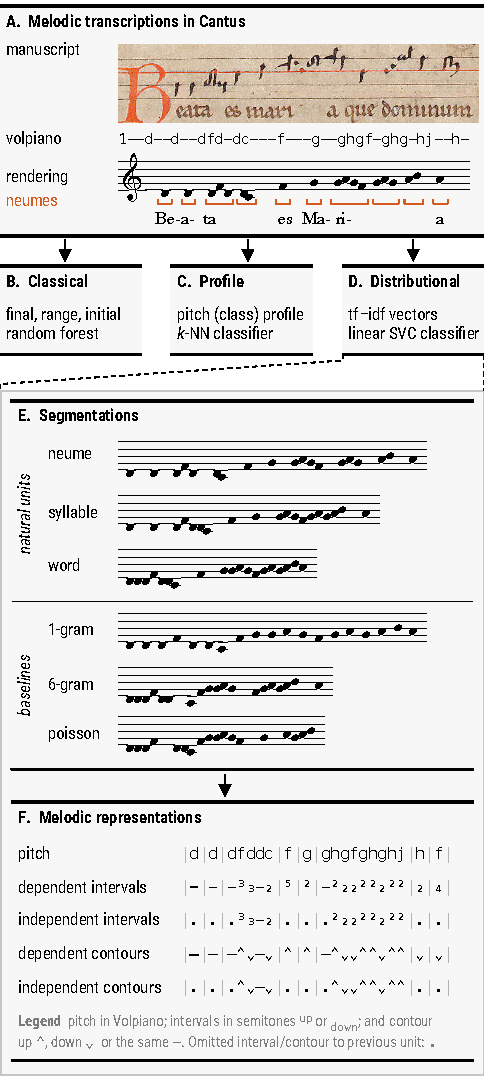
\includegraphics{figs/fig01-overview.pdf}
    \caption{
        \textbf{Overview of this study}
        %
        which compares three approaches to mode classification in a corpus of Gregorian chant.
        Cantus contributors have transcribed a vast number of melodies from medieval manuscripts \subfiglabel{a}.
        We classify mode based on the final, range and initial in the \emph{classical approach} \subfiglabel{b}, and based on pitch (class) and repetition profiles in the \emph{profile approach} \subfiglabel{c}.
        Finally in the \emph{distributional approach} \subfiglabel{d}, we use tf--idf vectors where we tweak two parameters: the \emph{segmentation}, or which melodic units we use \subfiglabel{e}, and the \emph{representation} \subfiglabel{f}, where we gradually discard information about the scale when we move from pitches to contours.
        In this way we aim to capture the melodic, rather than scalar, aspect of mode.
        %
        \label{fig:overview}
    }
\end{figure}
%-----------



%================
\section{Methods}
%================



The design of this study is visualized in \figref{fig:overview}.


\subsection{Data: the Cantus Database}
%-------------------------------------

We use chant transcriptions from the Cantus database \cite{Cantus}.
This is primarily a digital index of medieval chant manuscripts, recording the chant location in the manuscript, its full text, and properties like the mode, the liturgical feast, but also links to manuscript images.
Cantus currently consists of almost 150 manuscripts, containing over 450,000 chants, contributed by chant scholars from all over the world.
Over 60,000 chants also contain melodic transcriptions written in Volpiano.\footnote{
    %
    Volpiano is a typeface developed by David Hiley and Fabian Weber for notating plainchant. See \url{fawe.de/volpiano/}
    }
It sets plain text as musical notes on a five-line staff, as illustrated in \figref{fig:overview}a.
Volpiano also supports some accidentals, clefs, liquescents, barlines and strokes.
All submissions to Cantus are subject to strict guidelines and manually checked by the Cantus editors (see also \cite{Helsen2011}).
This ensures the quality and consistency of database, making it a valuable resource for computational research. 


We scraped the entire database of 497,071 chants via its \textsc{rest api} and we have released this as the CantusCorpus.\footnote{%
    %
    See \href{https://github.com/bacor/cantuscorpus}{github.com/bacor/cantuscorpus}, here we use v0.2.
    }
We here only consider chants that have a Volpiano transcription (63,628 chants) and 
further filter out chants with incomplete or non-standard transcriptions, without a complete melody, without `simple' mode annotation, and exact duplicates (see section \ref{suppl:filtering}).
This resulted in 7031 responsories (966,871 notes, avg.~length 138 notes) and 13,865 antiphons (825,143 notes, avg.~length 60 notes).
We fixed a 70/30 train/test split for all datasets and only used training data in exploratory analyses.
Cantus often contains multiple variants of any particular melody, transcribed from different manuscripts (see \figref{suppl:melody-variants}). 
One may wonder whether the simple train/test split is sufficient, or whether even more care is needed to avoid overlap between such melodic variants in the train and test sets.
This is a difficult issue that also applies to other musical corpora (e.g., the Essen folk-song corpus), and for which there is no perfect solution.
We tried repeating our experiments on a subset without variants and return to this issue in section~\ref{sec:melodic-variants}.


According to the transcription guidelines, flat symbols are transcribed only once, directly before the first flattened note.
We replace the first and later flattened notes by the corresponding accidental, a Volpiano character that sits at a specific staff line. 
In this way, flat notes are also encoded by a single Volpiano character.
We discard characters like clefs and pausas, and only retain the notes, accidentals and boundaries (hyphens).
The resulting string is used in our three classification experiments, which we now discuss.



%-----------------
\begin{figure}
    \centering
    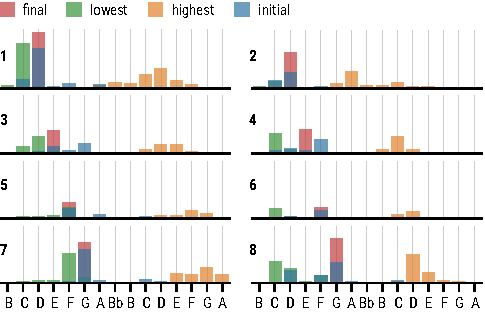
\includegraphics[width=8.2cm]{figs/fig02-classical-features.pdf}
    \caption{%
        \textbf{Classical features.}
        %
        The classical approach uses the final, range and initial to determine the mode.
        The overall distribution for each of the modes (1--8) is clearly different, although not entirely without ambiguity.
        %
        \label{fig:classical-features}
    }
\end{figure}
%-----------------
\begin{figure}
    \centering
    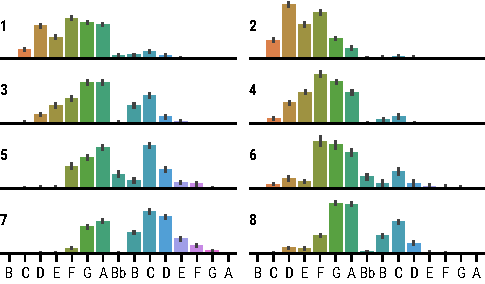
\includegraphics[width=8.2cm]{figs/fig03-pitch-profiles.pdf}
    \caption{%
        \textbf{Pitch profiles}
        %
        showing the relative frequency of every pitch in each of the 8 modes.
        Again, although the distribution of individual modes are clearly distinct, some residual ambiguity remains.
        %
        \label{fig:pitch-profile}
    }
\end{figure}
%-----------------
\begin{figure}
    \centering
    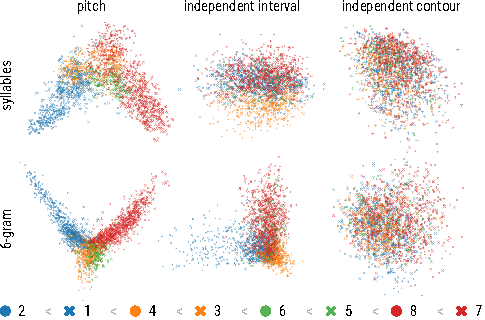
\includegraphics[width=8.2cm]{figs/fig04-pca-embeddings.pdf}
    \caption{%
        \textbf{\textsc{pca} of tf--idf vectors.}
        %
        Principal component projection of the tf--idf vectors of responsories in several conditions.
        The figure suggests that classification gets harder when moving from a pitch to a contour representation.
        The legend shows a theoretical ordering of the modes based on their range. See \figref{suppl:pca-plots} and \figref{suppl:t-sne-plots} for larger plots.
        %
        \label{fig:embeddings}
    }
\end{figure}
%-----------------


\subsection{Classical Approach: Final, Range, Initial}
%-------------------------------------------------------

The first approach is motivated by the classical procedure for mode classification.
We extract three features from every chant: the final pitch, the range (lowest and highest pitches) and the initial pitch.
Theory suggests that the final alone should give an accuracy of roughly 50\%, and adding the range should further increase that by roughly 50\%, if there is no ambiguity.
\figref{fig:classical-features} shows the feature distributions for all modes. 
It suggests that there is some ambiguity, and so numbers will be a little lower.
For this task we use random forest classifiers \cite{Breiman2001}, which aggregate multiple decision trees. 
Training details of all models are discussed below.



\subsection{Profile Approach: Pitch (Class) Profiles}
%--------------------------------------------

The second approach is inspired by Huron \& Veltman \cite{Huron2006a}.
Using 97 chants from the Liber Usualis, they compute average \emph{pitch class profiles} (the relative frequency of each pitch class) for each of the modes and then classified chants to closest profile.
We take a similar approach and use $k$-nearest neighbour classification, where $k$ is tuned (see section \ref{sec:training}).
In a commentary, Wiering \cite{Wiering2006} argued for using actual pitches rather than pitch classes, as the pitches an octave above the final have a very different role than those an octave below it. 
We follow that suggestion by also computing \emph{pitch profiles} (\figref{fig:pitch-profile}).
Finally, we propose a \emph{repetition profile} aiming to describe which notes function like a recitation tone.
For every Volpiano pitch $q$ we compute a repetition score $r(q)$, which is the relative frequency of direct repetitions, and collect these to get a repetition profile.
Formally, if a chant has pitches $p_1, \dots, p_N$, then
$r(q) = \#\{i: p_i = q \text{ and } p_{i+1} = q \} / (N-1)$  since there are $N-1$ possible repetitions.



\subsection{Distributional Approach: tf--idf Vectors}\label{sec:tfidf}
%----------------------------------------------------

Our third approach aims to capture the melodic aspect of mode.
In short, we use a bag of `words' model (cf.~\cite{Gulati2016a}) and tweak two parameters: the segmentation (which melodic units to use as `words') and the representation (pitches, intervals and contours).
The idea is to discard more and more information about the scale, and see if we can nevertheless determine the mode.


% Segmentations
% -------------
First, the units.
For chant, three natural segmentations suggest themselves: one can segment the melody (1) at neume boundaries, but also wherever we find (2) a syllable or (3) a word boundary in the lyrics.
Given the close relation between text and music in chant, there is some reason to believe that these are meaningful units.
Conveniently, all of these boundaries are explicitly encoded in Volpiano, by a single, double and triple dash respectively.
Note that these natural units are nested: neumes never cross syllable boundaries.
We compare the natural units to two types of baselines.
The first is an $n$-gram baseline where we slice the melody after every $n$ notes, for $n=1, \dots, 16$.
The second is a random, variable-length baseline.
Here the melody is segmented randomly, but in such a way that the segment length is approximately Poisson distributed with a mean length of 3, 5, or 7.
We stress that all these units are proper segmentations: units do not overlap. 
In particular, we choose not to use a higher-order model (using $n$-grams of units), because we are only interested in comparing different segmentations.


% Representations
% ---------------
Second, the representation.
We represent melodies in three ways: as a sequence of \emph{pitches}, \emph{intervals} (the number of semitones between successive notes) and \emph{contours} (the contour between successive notes: up, down or level).
There is one complication when segmenting sequences of intervals or contours: we introduce dependencies between the units.
All units would, for example, start with the interval from the previous unit. 
We call this a \emph{dependent} segmentation.
Alternatively, you could discard the intervals between units to obtain an \emph{independent} version.
This effectively makes every unit one interval shorter.
We analyse both independent and dependent versions, but in the independent one we found it convenient to start all units (including the first) with a dot to keep the segmentation identical across representations.
You can think of the dot as marking the omitted interval to the previous unit.


% Model
% -----
Third, the model.
Given a segmentation, we represent every chant by a vector of unit frequencies, but weighted to favour frequent, yet \emph{specific} units: units that do not occur in too many chants.
A standard way of doing this in textual information retrieval is using \emph{term-frequency inverse-document-frequency} (tf--idf) scores, which multiply the frequency of a term in a document (tf) by the inverse document frequency (idf): the inverse of the number of documents containing the term.
We use +1 smoothing for the idf, at most 5000 features, and found it was important \emph{not} to set a minimum or maximum document frequency.
We train a linear support vector machine to classify mode using the resulting tf--idf vectors.


In sum, we analyse 22 segmentations (3 natural ones, 16 $n$-grams, 3 random) and 5 representations (pitch and dependent/independent interval/contour), giving a total of 110 conditions.



\subsection{Training}\label{sec:training}
%--------------------

We tune every model using a randomised hyperparameter search with 5-fold stratified cross-validation. That is to say that we randomly sample hyperparameters from a suitable grid (determined by extensive manual analyses) and determine their performance using 5-fold cross-validation on the training set, where we ensure the class frequencies are similar in all folds. We use the hyperparameters yielding the highest cross-validation test accuracy to train the final model.
All models were implemented in Python using scikit-learn \cite{scikit-learn} and data and code are available online.\footnote{%
    %
    See \href{https://github.com/bacor/ISMIR2020}{github.com/bacor/ismir2020}
}




% %-----------------
\begin{figure*}[t!]
    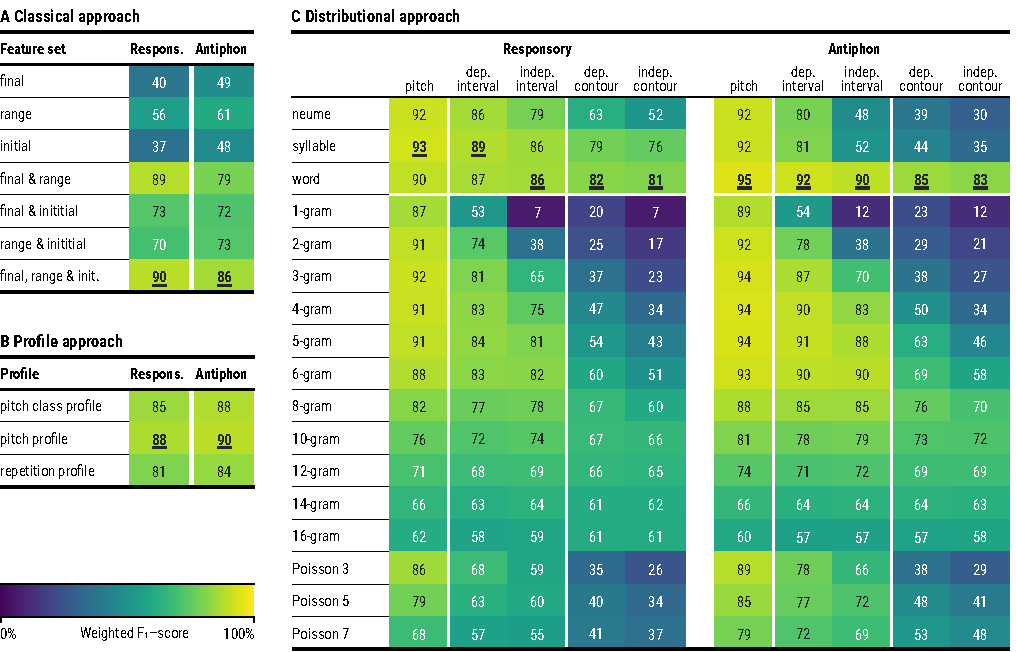
\includegraphics[width=\textwidth]{figs/fig05-classification-results.pdf}
    \caption{
        \textbf{Classification results.}
        %
        Weighted $F_1$-score for three approaches to mode classification, using two chant genres: responsories and antiphons.
        Scores are averages of five independent runs of the experiment.
        The classical approach \subfiglabel{A} using the final, range and initial reaches $F_1$-scores of 90\% and 86\%.
        The profile approach \subfiglabel{B} works better for antiphons (90\% vs.~86\%) and somewhat worse for responsories (88\% vs.~90\%).
        As \cite{Wiering2006} suspected, pitch profiles outperform pitch \emph{class} profiles by a small margin.
        The distributional approach \subfiglabel{C} reaches the highest $F_1$ scores of 95\% on both responsories and antiphons.
        The choice of segmentation (vertically) is crucial: classification is improved by using `natural' units, word-based units in particular, rather than $n$-grams.
        As the representation (horizontally) becomes cruder, from pitches to intervals and finally to contours, the task becomes much harder.
        But, when using word-based segmentation, performance remains high. 
        %
        \label{fig:scores}
    }
\end{figure*}
%-----------------



%================
\section{Results}
%================


Figure \ref{fig:scores} gives support-weighted\footnote{%
    %
    The retrieval scores for all classes (modes) are averaged, weighted by the number of instances in each class.
    }
averages of $F_1$-scores obtained on the full test sets for all three approaches.
The scores are averages of five independent runs of the experiment, using different train/test-splits.
Standard deviations were small and are included in figure \ref{suppl:results-full-stddev}.
We now compare the three approaches and then discuss the effect of representation and segmentation on the distributional approach.


\subsection{Approaches: Distributional Approach Works Best}
%----------------------------------------------------------

First of all, we report the highest classification scores with our distributional approach using pitch representations: an $F_1$-score of 93\% for responsories and 95\% for antiphons.
This corresponds of an error reduction of 30--60\% compared to the classical approach (90\% and 86\%).
The classical approach confirms the rule of thumb: the range and final are very informative features.
Using only these, we obtain $F_1$-scores of 89\% and 79\%, which are further increased by also adding the initial.
The profile approach outperforms the classical approach for antiphons (90\% vs.~86\%), but is outperformed for responsories (88\% vs.~90\%).
Our results support Wiering's \cite{Wiering2006} intuition that pitch profiles more accurately describe mode than pitch \emph{class} profiles, but the effect is small: it increases $F_1$ scores by 2--3\%.
Repetition profiles appear to be less useful for both genres.


In broad strokes, our results validate the classical and profile approach, both of which peak around a 90\% $F_1$-score, using simple features.
The distributional approach improves this, up to 95\% using complex features.
Importantly, we now show that the distributional approach maintains high performance when using interval or contour representations.



\subsection{Representations: Contours are Sufficient}
%----------------------------------------------------

We find that the classification task gets harder when the representation gets cruder, from those based on pitch, to intervals and finally to contours (figure \ref{fig:scores}C, horizontally).
This was anticipated: cruder representations are obtained by discarding information from every unit.
Shorter units are impacted more by this information loss.
For example, the performance with $1$-grams drops by over 75\% when moving from pitch to independent contour representation.
At that point it performs at majority baseline (a 7\% $F_1$-score for responsories and 12\% for antiphons).\footnote{%
    %
    For 1-grams in independent interval \emph{and} contour representation, every unit is identical: a dot representing the omitted contour to the previous note. 
    The majority class for both responsories and antiphons is mode 8, taking up 21\% and 28\% of the test data respectively (see table \ref{suppl:majority-baselines}).
    This is precisely the accuracy of the model in those conditions.
    }
For longer units such as $10$-grams, the drop is not as dramatic (around 10\%).
However, this comes at the cost of a comparatively low performance using the pitch-representation, presumably because of increasing sparsity.

Natural units, however, escape this trade-off.
Word-based segmentations perform consistently well, dropping only 3\% below the classical baseline using the highly impoverished independent contour representation.
In contrast to the other representations, the contours do not carry any information about the scale: the same contour can be reproduced in any scale.
Apparently, we can discard the scalar aspect of mode, and still classify it: contours alone contain sufficient information for mode classification.
The success of pitch-based methods might obscure the fact that mode is as much a melodic phenomenon as a scalar one.


It is interesting to note that the earliest chant notation used \emph{unpitched} neumes that mainly described the contour of the melody---not the exact pitches.
Our results reinforce the idea that contour is highly informative---so informative that given a mode, text and contour, an experienced singer could reconstruct the chant melody.




\subsection{Segmentations: Natural Units Work Best.}
%---------------------------------------------------

Our most important result is that among all the representations we considered, natural units (neume, syllables, and words) yield the highest classification performance.
The 4- and 6-gram baselines also reach top $F_1$-scores in antiphons, but only when we use representations that include information about pitch.
Furthermore, the success of natural units cannot be explained solely by their length.
In responsories, neumes, syllables and words are on average 2.3, 3.0 and 7.1 notes long, respectively (see table \ref{suppl:unit-lengths}), and yet the performance of these natural units is consistently higher than $n$-grams of comparable length. The performance of the natural units is also consistently higher than that of the variable-length Poisson baselines, which are intended to mimic the overall distribution of natural lengths but ignore musical and textual semantics.

A few other observations merit discussion.
Firstly, although neume and syllable segmentations behave differently for responsories, they behave similarly to each other for antiphons.
The reason may be that in antiphons, neumes and syllables more often coincide.
Antiphons are less \emph{melismatic} than responsories (i.e., they use fewer notes per syllable, 1.5 to be precise).
Secondly, both the $n$-grams and the Poisson baseline perform better on antiphons than on responsories, possibly because the $n$-grams are more likely to end up being coincidentally aligned with the natural units the less melismatic the genre.




\subsection{Controlling for Melodic Variants}\label{sec:melodic-variants}
%--------------------------------------

We repeated all experiments on a subset of the data from which we removed melody variants (see supplement \ref{suppl:results-subset} for details).
In terms of the number of notes, this meant a 75\% and 66\% reduction in data size for responsories and antiphons respectively.
The performance of all models decreased on this subset, and for responsories more than for antiphons.
Our main findings that contours are sufficient and that natural units work best across representations stand.
We do observe some reorderings: some already high-performing $n$-grams in antiphons now for example slightly overtake word segmentations, although only for pitch and dependent interval representations.
The distributional approach works best for antiphons regardless of including or excluding chant variants, but for responsories, the distributional approach drops slightly below the classical approach on the subset (where the profile approach is worst).
These findings might be explained by increased sparsity in the smaller dataset: natural units in responsories are, after all, longer.
Exploring these issues further is left for future work.



%====================
\section{Discussion and Conclusion}
%====================


In this paper, we analyzed three approaches to mode classification in a large corpus of plainchant: (1) the classical approach using the final, range and initial; (2) the profile approach using pitch (class) profiles and (3) the distributional approach using a tf--idf vector model and various segmentations and representations.
We found that the distributional approach performs best, and that it can maintain high performance on contour representations if using the right segmentation: at word boundaries, in this case.
The main findings were largely upheld when we removed melody variants, but the handling of variants is an issue that deserves further investigation and that has implications beyond this study.

Although our results are specific to one corpus of medieval music and one classification task, we believe our conclusions are of wider relevance. 
We often fall back on $n$-grams because they are well understood and easy to use. A more natural segmentation may be harder to obtain, but if finding them can have such a large effect on a relatively simple task like mode classification, their advantages may be even stronger for more complex tasks. 


A first next step could be to explore whether lyrics yield equally useful units in other vocal musics.
As noted, the link between text and music in plainchant is particularly tight.
This at least suggests that the text may be useful in other types of chant, like Byzantine chant or Torah trope.
For folk melodies designed to standard poetic meters, it is not as obvious whether lyrics would help or hinder the identification of useful units.
This is worth investigating, as characteristic motifs and repeated pattern are commonly used in computational folk-song studies, in particular for tune family identification \cite{Volk2012,Janssen2017a}.


Our results raise another question: is chant indeed composed by stringing together certain melodic units, much like a sentence is composed of words?
It has been suggested (and disputed) that Gregorian chant is composed in a process of \emph{centonization}, and that a chant is a patchwork of existing melodic chunks called \emph{centos}.
A recent study used the tf--idf weighting to discover centos in  Arab-Andalusian music \cite{Nuttall2019}.
This raises the possibility that classification using natural units may have been successful because they indeed are the building blocks, the centos.


Chant is not yet commonly studied in the \textsc{mir} community, but we hope that this study shows that chant is an interesting repertoire that can yield insights of broader relevance. 
The immense efforts of chant scholars mean that data are abundant.
In short, we think chant can aid the development of models that apply beyond Western classical and pop music, and embrace the true diversity of musics around the world.

\bibliography{references}







%%%%%%%%%%%%%%%%%%%%%%%%%%%%%%%%%%%%%%%%%%%%%%%%%%%%%%%%%%%%%
%%%%%%%%%%%%%%%%%%%%%%%%%%%%%%%%%%%%%%%%%%%%%%%%%%%%%%%%%%%%%
%%%%%%%%%%%%%%%%% S U P P L E M E N T S %%%%%%%%%%%%%%%%%%%%%
%%%%%%%%%%%%%%%%%%%%%%%%%%%%%%%%%%%%%%%%%%%%%%%%%%%%%%%%%%%%%
%%%%%%%%%%%%%%%%%%%%%%%%%%%%%%%%%%%%%%%%%%%%%%%%%%%%%%%%%%%%%





\clearpage
\onecolumn
\setcounter{figure}{0}
\renewcommand{\thefigure}{S\arabic{figure}}%

% Supplements header
\begin{center} 
    {\Large \bf \uppercase{Supplements} \\[.5em]}
    {\Large Mode Classification and Natural Units in Plainchant}
    \\[.5em]
    {\large Bas Cornelissen, Willem Zuidema and John Ashley Burgoyne}
\end{center}

\vspace{2em}

\noindent
\textbf{Data and code.}
All data and code used in this study has been made available online at \href{https://github.com/bacor/ISMIR2020}{github.com/bacor/\textsc{ismir2020}}.
All randomness in the code has been fixed, so it should in theory be possible to reproduce our results exactly.
The evaluations metrics of all experiments are already included in the repository, as is the data used in the first run of the experiment; this should be sufficient for reproducing most figures.
We have included model predictions and tuning results only for the first run of the experiment. 
Detailed logs of everything from data generation to vizualization can also be in the repository, together with many more figures besides those included in the paper and the supplements. 
In particular, the repository contains heatmaps with multiple evaluation metrics (accuracy, precision, recall and $F_1$) for all models and all experimental conditions.


\begin{figure*}[b!]
\begin{framed}
\small
\begin{verbatim}
Filtering chants...
. Filter Chants Without Volpiano:
. Exclude all chants with an empty volpiano field
.  > 87.20% removed (433443 out of 497071; 63628 remain)
. Filter Chants Without Notes:
. Exclude all chants without notes
.  > 2.87% removed (1825 out of 63628; 61803 remain)
. Filter Chants Without Simple Mode:
. Include only chants with simple modes: 1-8, not transposed
.  * include_transposed=False
.  > 23.02% removed (14227 out of 61803; 47576 remain)
. Filter Chants Without Full Text:
. Filter chants without full text
.  > 20.65% removed (9823 out of 47576; 37753 remain)
. Filter Chants Where Incipit Is Full Text:
. Filter chants whose incipit is identical to the full text
.  > 14.59% removed (5507 out of 37753; 32246 remain)
. Filter Chants By Genre:
. Include only chants with a certain genre
.  * include=['genre_a']
.  > 52.06% removed (16787 out of 32246; 15459 remain)
. Filter Chants Not Starting With G Clef:
. Exclude chants that do not start with a G clef
.  > 0.05% removed (7 out of 15459; 15452 remain)
. Filter Chants With F Clef:
. Exclude chants that contain an F clef
.  > 0.00% removed (0 out of 15452; 15452 remain)
. Filter Chants With Missing Pitches:
. Filter chants with missing pitches: containing the substring 6------6
.  > 7.54% removed (1165 out of 15452; 14287 remain)
. Filter Chants With Nonvolpiano Chars:
. Exclude all chants with non-volpiano characters
.  > 0.03% removed (5 out of 14287; 14282 remain)
. Filter Chants Without Word Boundary:
. Only include chants with '---' in their volpiano
.  > 0.08% removed (11 out of 14282; 14271 remain)
. Filter Chants With Duplicated Notes:
. Filter duplicate chants: whose notes occur multiple times
.  > 2.84% removed (406 out of 14271; 13865 remain)
\end{verbatim}
\end{framed}
    \caption{
        \textbf{Filtering.}
        As described in the main text, we filtered the total dataset of 497,071 chants to obtain a clean subset of responsories and antiphons.
        The effects of all of the filters are logged and will be made available online.
        As an example, this `figure' shows the series of filters applied to obtain the full set of antiphons used in this study.
        \label{suppl:filtering}
    }
\end{figure*}


\begin{figure*}
\centering
\begin{tabular}{@{}lllrrr@{}}
\toprule
Genre      & Subset & Split & \# chants & \# notes & Mean length (notes) \\ \midrule
responsory & full   & train & 4 922  & 676 807     & 137.5  \\
responsory & full   & test  & 2 109  & 290 064     & 137.5  \\
responsory & full   & total & 7 031  & 966 871     & 137.5  \\
responsory & subset & train & 1 234  & 169 642     & 137.5  \\
responsory & subset & test  & 529   & 72 504      & 137.1  \\
responsory & subset & total & 1 763  & 242 146     & 137.3  \\
antiphon   & full   & train & 9 706  & 576 738     & 59.4   \\
antiphon   & full   & test  & 4 159  & 248 405     & 59.7   \\
antiphon   & full   & total & 13 865 & 825 143     & 59.5   \\
antiphon   & subset & train & 2 911  & 190 165     & 65.3   \\
antiphon   & subset & test  & 1 248  & 82 781      & 66.3   \\
antiphon   & subset & total & 4 159  & 272 946     & 65.6    
\\ \bottomrule
\end{tabular}
\caption{\textbf{Dataset statistics.} The number of chants, their average length and number of notes for each dataset. We sort datasets by genre, then by subset (include melody variants in the full set, or exclude them in the subset) and finally by train/test split (or total for the two combined).
The train/test splits are different in each run of the experiment. These statistics are computed from the data used in the first run, and others are comparable.
}
\label{suppl:dataset-statistics}
\end{figure*}



\begin{figure*}
\centering
\begin{tabular}{lllll} \toprule
genre      & dataset & kind  & top mode & frequency \\ \midrule
responsory & full   & train & 8     & 20.85\% \\
responsory & full   & test  & 8     & \textbf{21.13}\% \\
responsory & subset & train & 1     & 21.65\% \\
responsory & subset & test  & 1     & 20.19\% \\
antiphon   & full   & train & 8     & 28.47\% \\
antiphon   & full   & test  & 8     & \textbf{28.13}\% \\
antiphon   & subset & train & 1     & 23.50\% \\
antiphon   & subset & test  & 1     & 24.18\% \\
\bottomrule
\end{tabular}
\caption{\textbf{Majority baselines}. The frequency of the largest classes in each of the datasets. Boldfaced values correspond to the classification \emph{accuracy} of the worst-performing conditions discussed in the main text. (The frequencies are marginally different in the five experimental runs; shown are the averages.)}
\label{suppl:majority-baselines}
\end{figure*}


\begin{figure*}
    \centering
    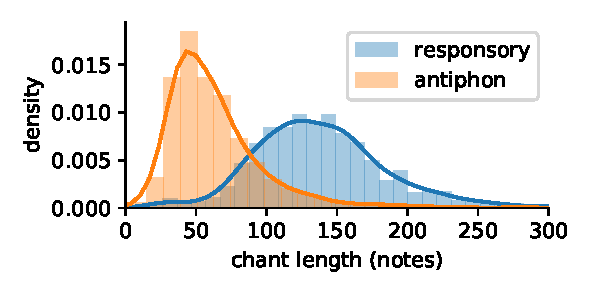
\includegraphics[width=.4\textwidth]{figs/figS03-chant-length-distribution.pdf}
    \caption{
        \textbf{Chant lengths in two genres.}
        Responsories are usually much longer than antiphons. The distribution is estimated from the training datasets without melody variants.
        \label{suppl:chant-length-distributions}
    }
\end{figure*}


\begin{figure*}
    \centering
    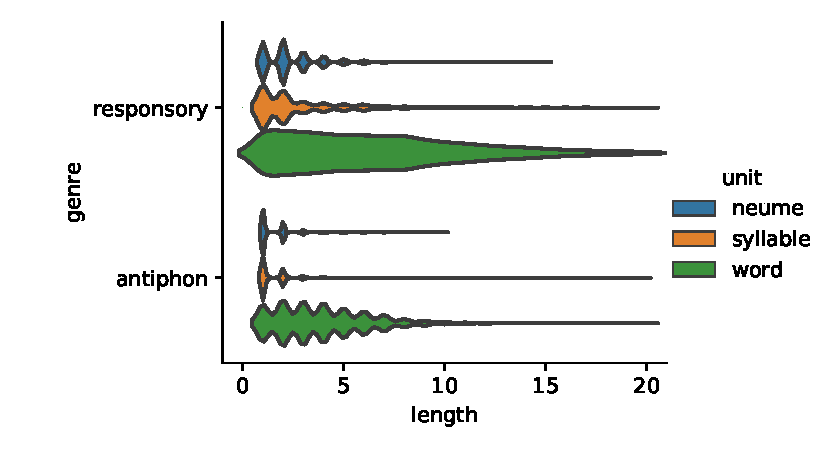
\includegraphics[width=.6\textwidth]{figs/figS06-unit-length-distribution.pdf}
    \caption{
        \textbf{Lengths of natural units.}
        Natural units have different lenghts in responsories and antiphons.
        Responsories are more \emph{melismatic}: they use more notes per syllable.
        As a result, a typical word is also much longer.
        This is shown in the figure using violin plots, a visualization of the length distribution using a kernel density estimate. Note that the total area has no meaning in this plot; we normalized the widths of the violins for better readability. 
        The distributions are estimated from the training datasets without melody variants).
        \label{suppl:unit-length-distributions}
    }
\end{figure*}

\begin{figure*}
    \centering
    \begin{tabular}{llll}\toprule
               & neume & syllable & word \\\midrule
    antiphon   & 1.50 & 1.55 & 3.98 \\
    responsory & 2.32 & 2.96 & 7.12 \\ \bottomrule
    \end{tabular}
    \caption{
        \textbf{Mean lengths of natural units.} 
        Natural units have different lengths in responsories and antiphons, as the mean lenghts in number of notes shows. Figure \ref{suppl:unit-length-distributions} shows the full distribution.
        Means estimated from the training datasets without melody variants.
        \label{suppl:unit-lengths}
    }
\end{figure*}


\begin{figure*}
    \centering
    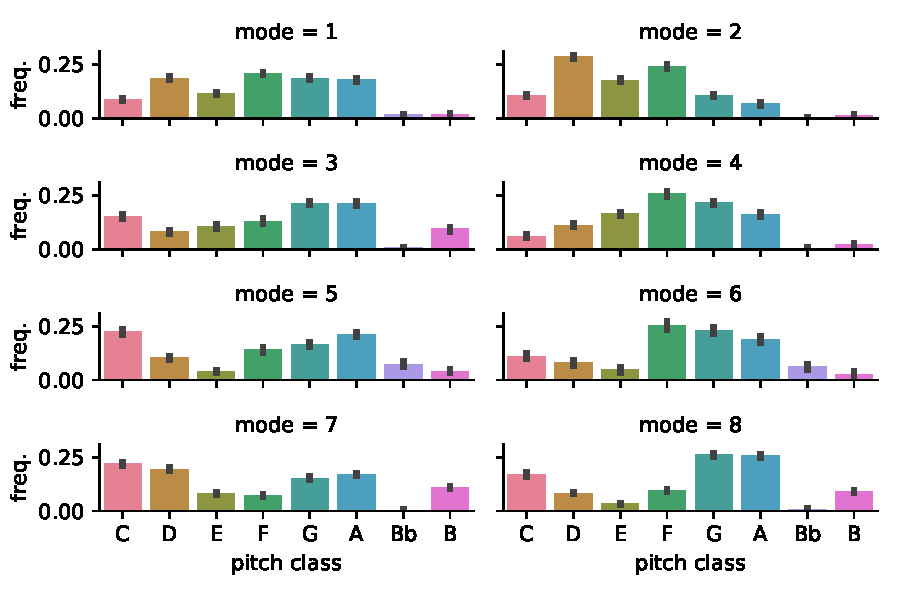
\includegraphics[width=.7\textwidth]{figs/figS07-pitch-class-profiles.pdf}
    \caption{
        \textbf{Pitch class profiles}
        %
        The pitch class profiles used in the profile approach (cf \cite{Huron2006a}). Shown are data for responsories, estimated from the training data without melody variants.
        \label{suppl:pitch-class-profiles}
    }
\end{figure*}

\begin{figure*}
    \centering
    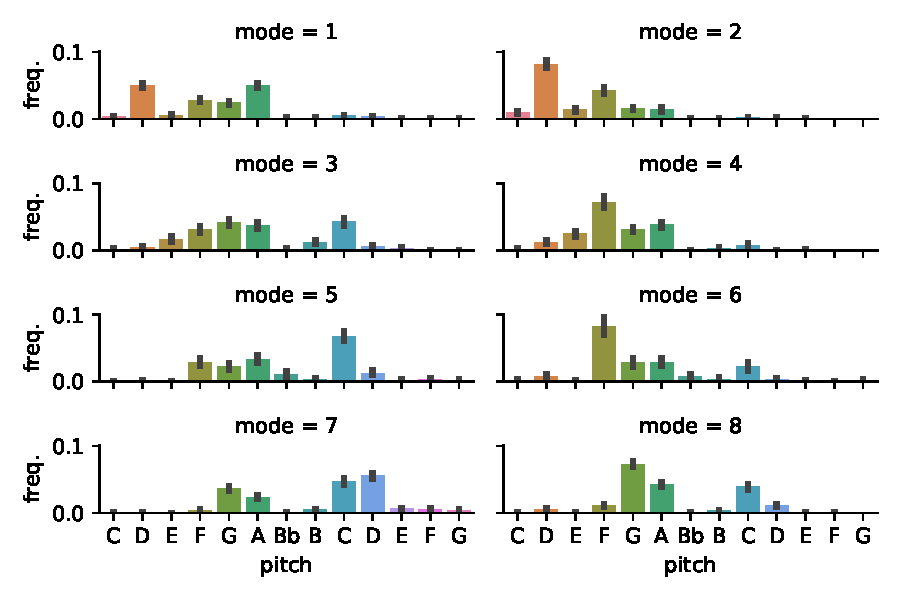
\includegraphics[width=.7\textwidth]{figs/figS08-repetition-profiles.pdf}
    \caption{
        \textbf{Repetition profiles}
        %
        The repetition profiles used in the profile approach.
        Every bar shows the average number of repetitions of that note in a chant (see main text for details).
        Shown are data for responsories, estimated from the training data without melody variants.
        \label{suppl:repetition-profiles}
    }
\end{figure*}




\begin{figure*}
    \centering
    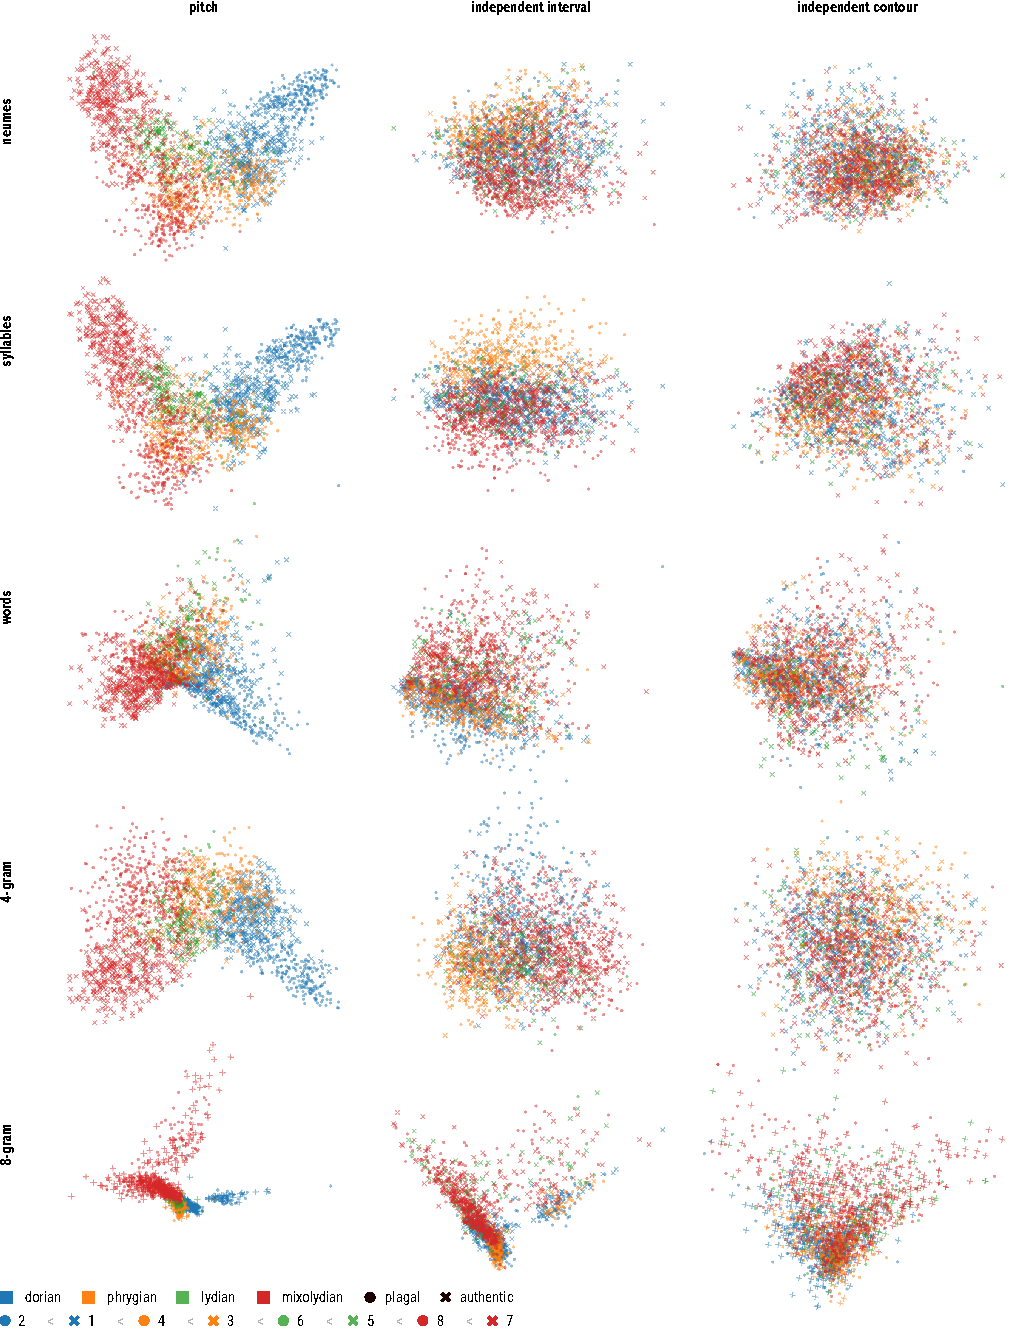
\includegraphics{figs/figS09-PCA-embeddings.pdf}
    \caption{
        \textbf{\textsc{pca} plots.}
        Two-dimensional representation of the high-dimensional feature space
        in several different conditions.
        A sample of \textsc{tf--idf} vectors is shown, after reducing their dimensionality using a principal component projection.
        \label{suppl:pca-plots}
    }
\end{figure*}




\begin{figure*}
    \centering
    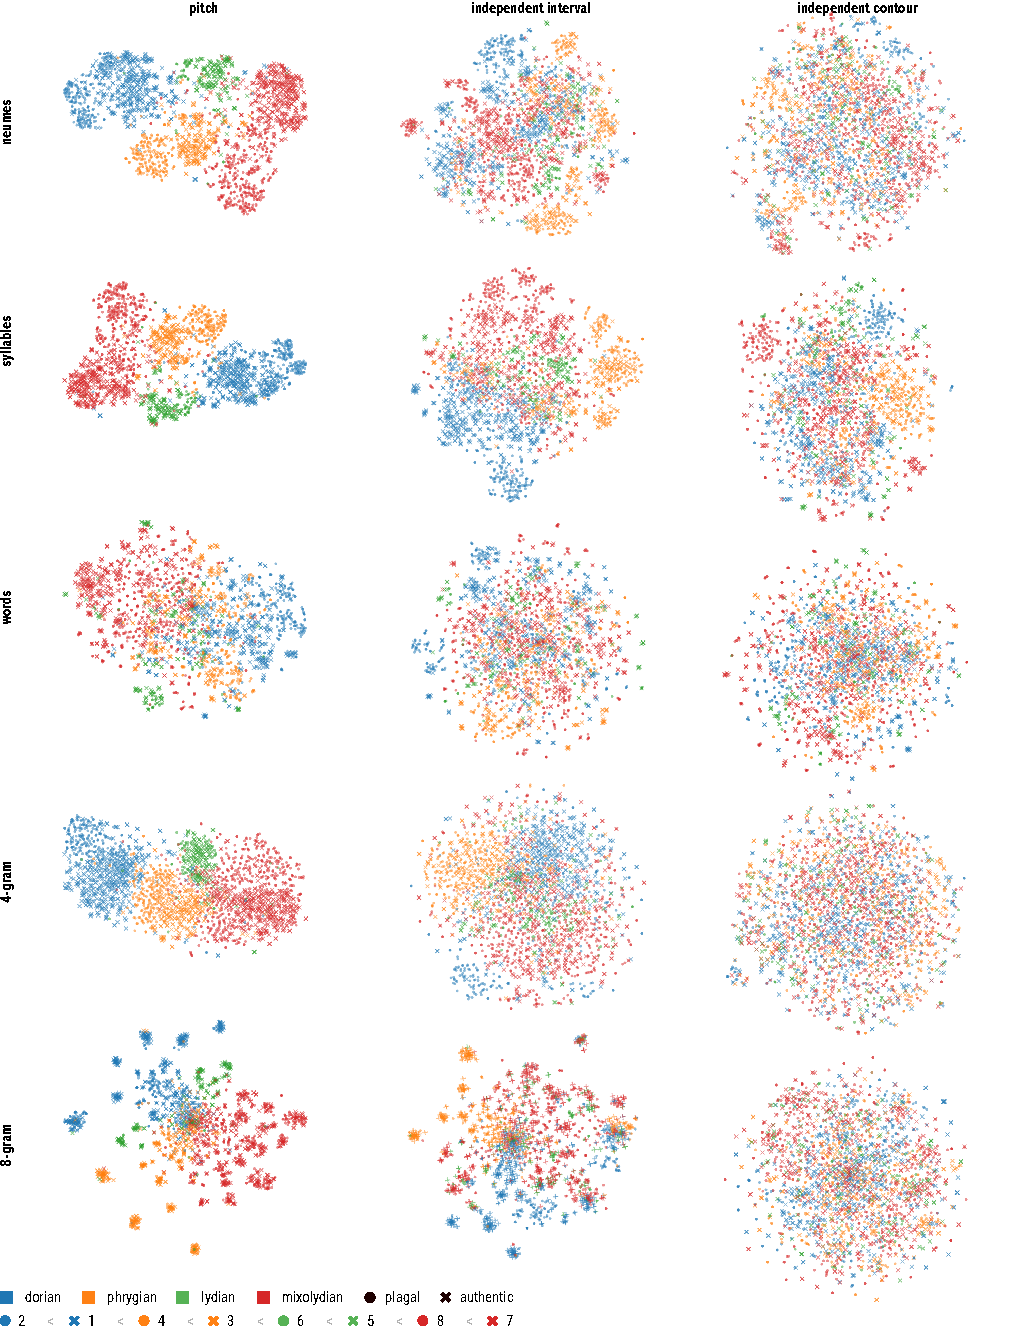
\includegraphics{figs/figS10-tSNE-embeddings.pdf}
    \caption{
        \textbf{$t$-\textsc{sne} plots.}
        Two-dimensional representation of the high-dimensional feature space
        in several different conditions.
        A sample of \textsc{tf--idf} vectors is shown, after reducing their dimensionality using $t$-\textsc{sne}, a nonlinear dimensionality-reduction technique that maximizes the probability of mapping nearby points in high-dimensional space to nearby points in a lower dimensional space. The axes have no natural interpretation, but the graphs suggest that clusters are most clearly separated at the left, and mostly overlapping at the right.
        \label{suppl:t-sne-plots}
    }
\end{figure*}




\begin{figure*}
    \centering
    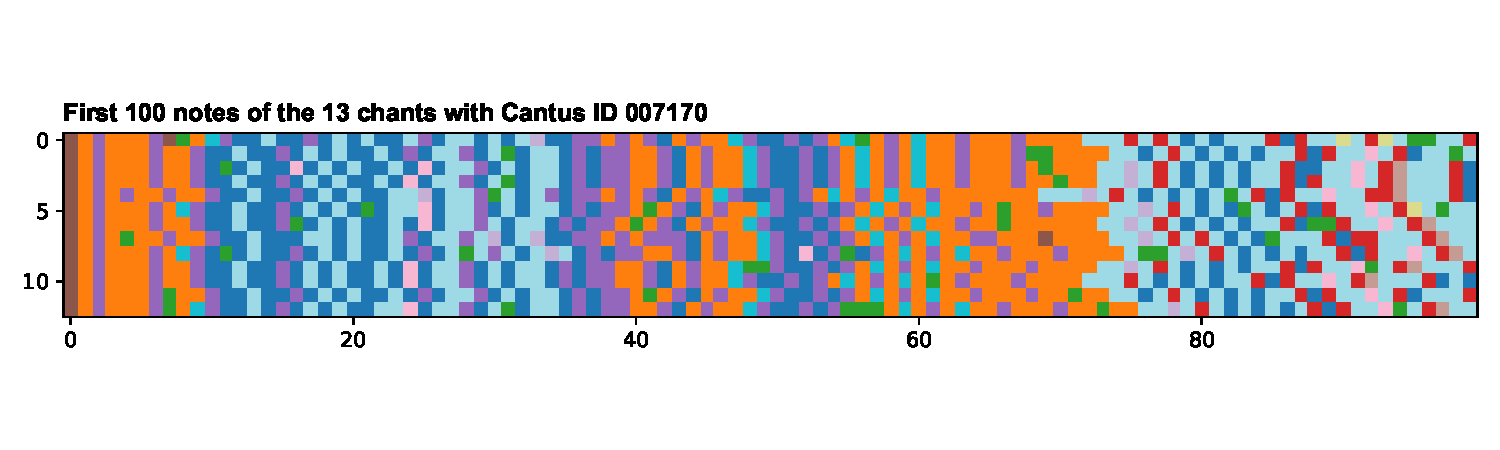
\includegraphics[width=\textwidth]{figs/figS11-melody-variants-0.pdf}
    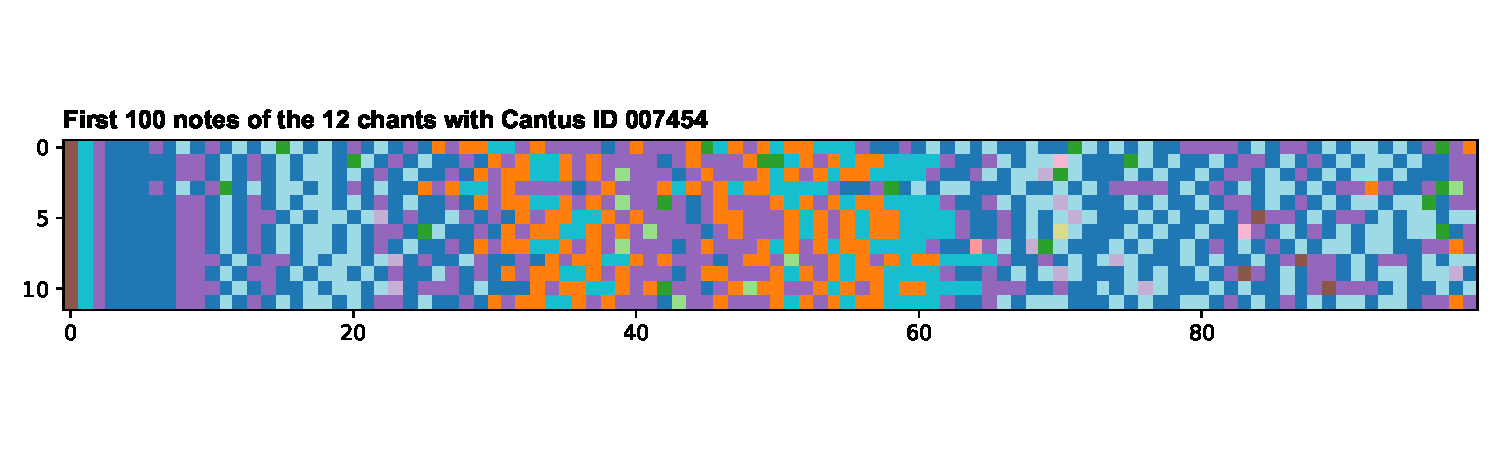
\includegraphics[width=\textwidth]{figs/figS11-melody-variants-1.pdf}
    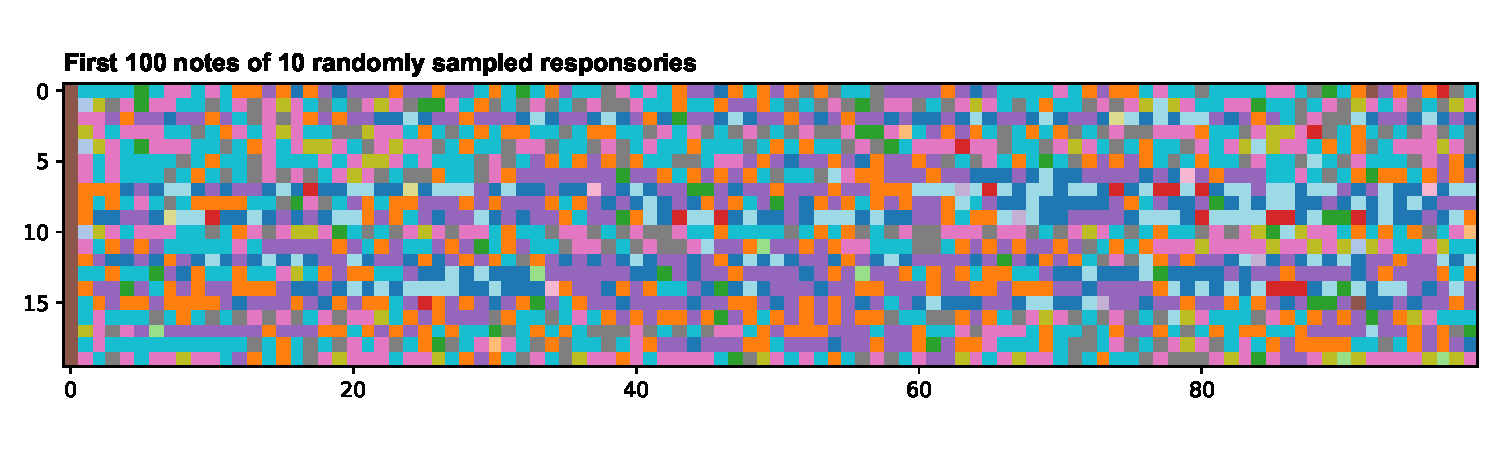
\includegraphics[width=\textwidth]{figs/figS11-melody-variants-random.pdf}
    \caption{
        \textbf{Melody variants in Cantus.}
        The top three panels show examples of sets of melody variants:
        the first 100 notes of melodies sharing a Cantus \textsc{id}. 
        Different colors correspond to different pitches, or more precisely, different Volpiano characters after discarding dashes.
        As a comparison, the bottom panel shows 100 notes of 20 random melodies.
        \label{suppl:melody-variants}
    }
\end{figure*}

\begin{figure*}
    \centering
    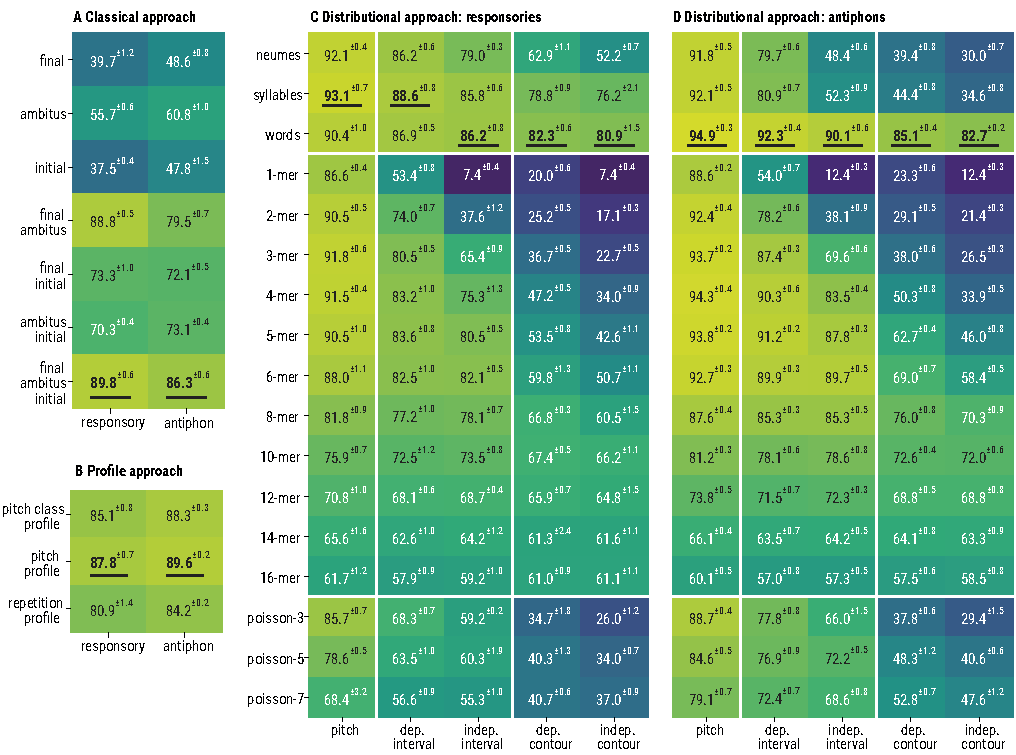
\includegraphics{figs/figS12-full-results-stddev.pdf}
    \caption{
        \textbf{Classification results with standard deviation.}
        This is essentially the same figure as figure \ref{fig:scores} but now with the mean $F_1$-score $\mu$ and its standard deviation $\sigma$ shown as $\mu^{\pm\sigma}$, computed from five independent runs of the experiment.
        \label{suppl:results-full-stddev}
    }
\end{figure*}


\begin{figure*}
    \centering
    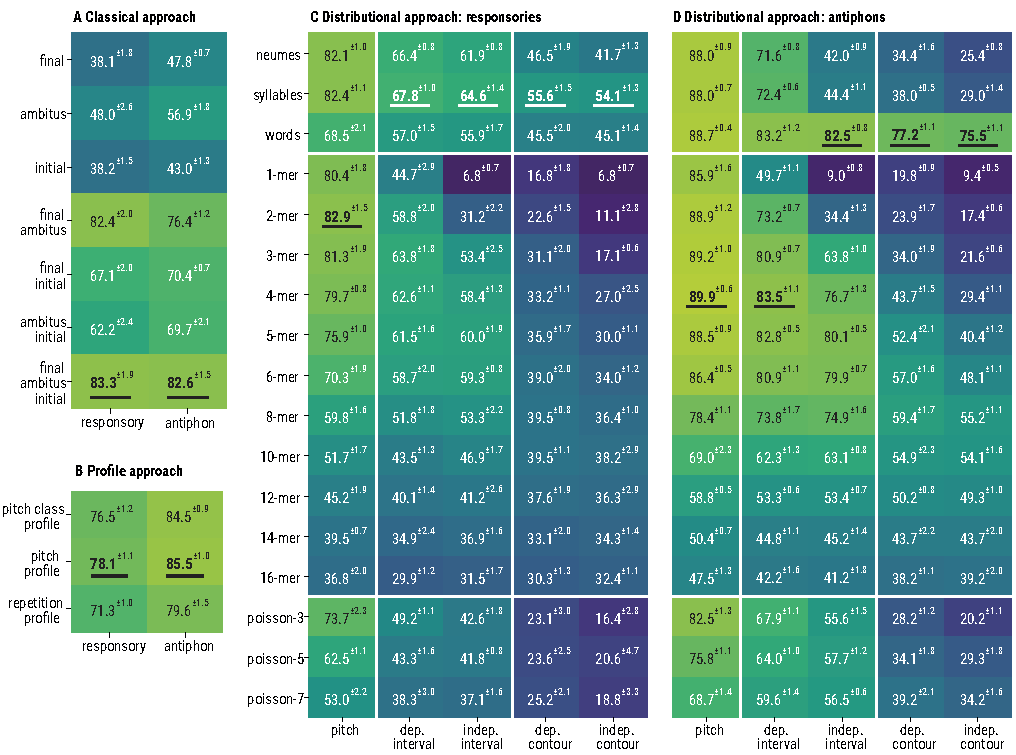
\includegraphics{figs/figS13-subset-results-stddev.pdf}
    \caption{
        \textbf{Main results on subset.}
        Cantus often contains several variants of the same melody, as shown in \figref{suppl:melody-variants}.
        As discussed in the main text, this is a difficult issue that for example also applies to the Essen folk-song collection.
        We decided to repeat our experiments on a subset of the data where we excluded melody variants.
        We heuristically identified melody variants by randomly picking one chant from all sets of chants that have the same Cantus \textsc{id} and mode.
        This resulted in a set of 1763 responsories and 4159 antiphons.
        This figure shows the main classification results on this subset of the data.
        Clearly, the performance of all models drops.
        The drop is greatest for responsories across models. 
        The main result that only natural units maintain high performance, even on contour representations, nevertheless stand.
        It should be noted that in antiphons, some $n$-grams now outperform the natural units (by less then 2\%) when using pitch and dependent interval representation.
        This does not reflect a large change in performance: in the main results, these $n$-grams are also deviated from top performance by no more than 2\%.
        These results are further discussed in the main text.
        \label{suppl:results-subset}
    }
\end{figure*}


\end{document}